%set the master document for easy compilation
%!TEX root = ../D3_5_3.tex

\chapter{Purpose of the document}

This document is managed as a deliverable of the modeling work package with denomination ~D3.7.x, and contains advices and recommendation for the design of a physical system architecture.  

The development of the functional model is done iteratively increasing the scope in steps, the last digit of the deliverable identifier, i.e.~x, denotes the release of the model to which it applies. If the functional model requires to update the system architecture a consistent version number will be applied to this document as required by the Model release version.

This document complements the indications contained in the API requirements specification and the documentation derived from this as the generic openETCS Application Programming Interface (API), available at \url{https://github.com/openETCS/modeling/blob/master/API/description/api-description.pdf}. \cite{alstom-api}

\section{Input Documents}

The following documents provide a context for the system perspective.

\begin{itemize}
	\item ERA Subset-026 \cite{subset-026}, V3.3.0
	\item ERA TSI CCS Documents
	\item openETCS API documentation, available at \url{https://github.com/openETCS/modeling/blob/master/API/description/api-description.pdf} \cite{alstom-api}\cite{alstom-api-app-layer}\cite{alstom-api-data-dict}
	%\item openETCS requirements, i.e.~D2.1, D2.2,$\ldots$, %D2.9, available at %\url{https://github.com/openETCS/requirements/tree/maste%r/Reference}
\end{itemize}




\chapter{Introduction}

Designing a sub system integrable with the train borne system is a complex task. The designer faces a large variety of serious challenges and design complexities. 

Before the functions are actually implemented, a system architect will have to select an appropriate hardware-software concept out of the large number of available boards, controllers, network and  bus constraints.  He  will as well include robustness criteria against environmental influences. 

Memories, operating systems, drivers, generic and application software segregation as well as selection criteria for sensors and actuators need to be correctly assessed. 

The target architecture has to meet a large variety of requirements. Criteria of timing, Bus bandwidth, processor and peripheral performance, memory size, safety principles and possible processing or data transfer bottlenecks. Environmental conditions, timing constraints, robustness against specific interferences shall constantly be tracked.

Power requirement as well as allocation of availability, maintainability figures to enumerate only the most relevant items accompany all the design phases.

On top of this a specific vital architecture has to be selected and the required integrity level has to be granted. The relative safety constraints have to be assured and maybe exported.

Selecting the components matching these is a critical phase. Over-dimensioning the architecture may impact on cost factors relevant for the market access of the system. Under-dimensioning the architecture design could result in not achieving performance constraints, thus compromising system quality and suitability. Early architectural choices have a dominant impact on the success of the new system. 

The system architects will commit to efficient design choices according to the target project margins and all this within the frame of a defined project delivery time schedule. 

Due to the fact that the design verification phase, requiring to have completed all the integration steps, may be very late in the release process a high precision during the system architecture design is mandatory. 

Therefore highly experienced System Designer are considered as the key factor for a reliable achievement of expected design result.

A primary goal of the openETCS ITEA2 project is to provide a formal specification and a model of an ETCS onboard functionality according to the specification defined in Subset-026 \cite{subset-026} by the European Railway Agency (ERA). 

The Model-Based Development process is an approach that allows engineers to specify the behavior of a system and to simulate and execute it in a very early development stage.

Once a model-based development process has been established, engineers should be able to apply new technologies and tools to enhance and shorten product development cycles,
e.g. by introducing generation of Model Validation test cases and target Code directly from the model. This enables to improve the V based development process to save development time and effort while preserving or improving the dependability of the developed systems. 


\begin{figure}[H]
	\center
	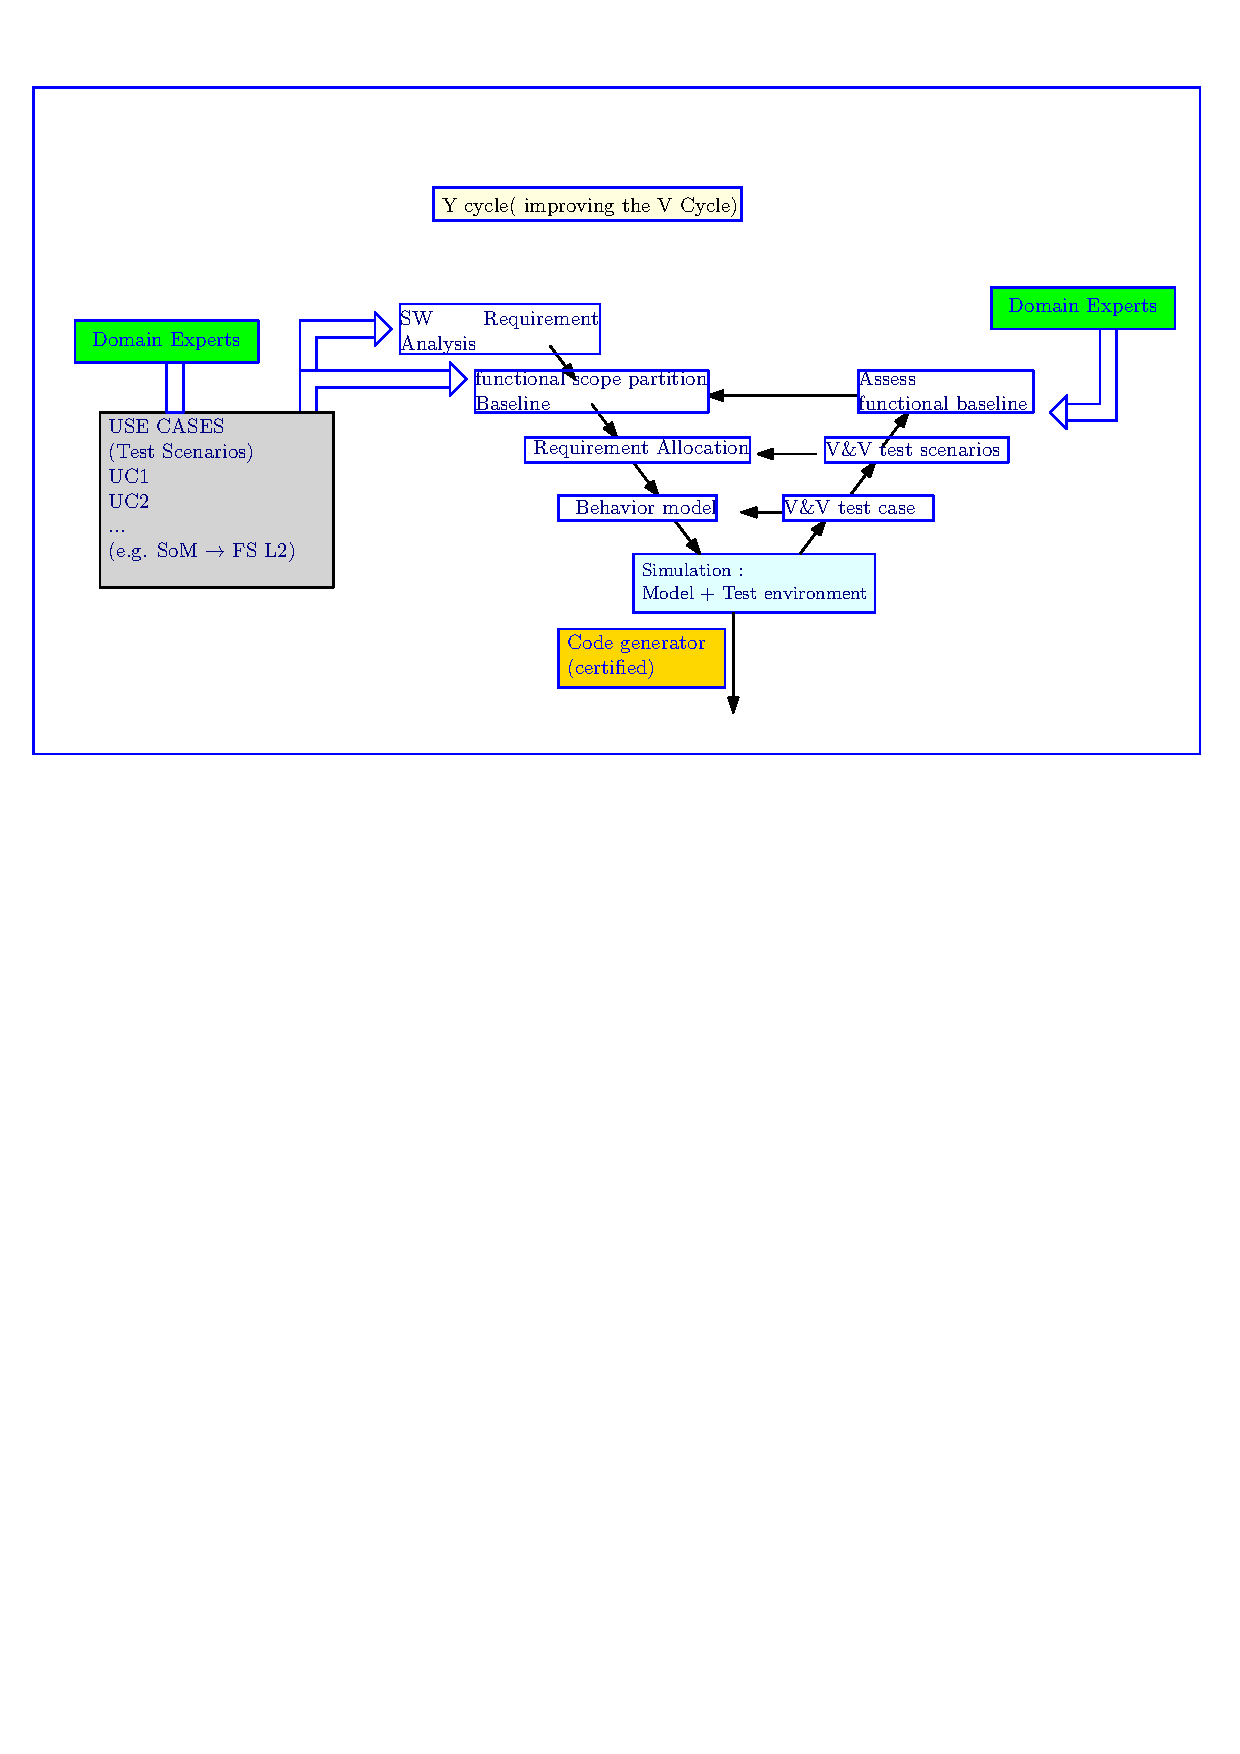
\includegraphics[width= 0.9\textwidth]{Y_process.pdf}
	\caption{SRS modeling cycle}\label{Y_process}
\end{figure}


The methodology makes it easier to understand requirements and increases the correctness of the requirements, the correctness of the design and the code with respect to the requirements. An integration of system-level and design-level modeling tools allows a virtually integrated V-process that is sharpened up to a Y-based process with the required steps at the bottom of the former V being considerably automated (see figure\ref{Y_process} )

Nevertheless when specifying the overall software architecture, the designer should be aware of the implications of software design decisions on the target end system.

\section{Safety Integrity and Functional Safety according CENELEC}
The Railway Industry currently relies on the international standard group of coordinated standards: EN 50126 “Railway
applications – The specification and
demonstration of Reliability, Availability,
Maintainability and Safety (RAMS)” 
the EN 50129 “Railway applications – Safety
related electronic systems for signalling” and
the EN 50128 “Railway applications -  Communications, signalling and processing systems – Software for railway control and  protection systems” to provide a rational and consistent approach for the development of safety-related systems.

This group of standards owes much of its direction and contents to the IEC 61508 standard that is a generic safety standard for electrical/electronic/programmable electronics safety-related systems.

Both of these IEC and EN standards share the same philosophy in the sense that they:

\begin{itemize}
\item consider all relevant product and software safety life-cycle phases, from an initial concept phase to maintenance and decommissioning when these systems are used to perform safety functions;
\item intend to shape a safety awareness; \item have been conceived with a rapidly developing technology in mind;
\item provide methods and rules for defining safety requirements necessary to achieve defined functional safety.
\item use Safety Integrity Levels (SIL) for specifying the target level of safety integrity for the safety functions to be implemented.
\item adopt a statistical risk-based approach for the determination of the SIL requirements;
\item distinguish between safe and unsafe failure modes and requires precautions against undetected failures. 
\end{itemize}

According the Cenelec norms the product is subject to a certification process. The definition of the equipment under control (EUC) depends on the scope of the certification. It can be, for example the complete ERTMS/ETCS subsystem or a  module of it.

The term safety-related is used to describe systems that are required to perform a specific function to ensure that risks are kept at an acceptable level. Such functions are, by definition, safety functions. Two types of requirements are necessary to achieve functional safety: 

\begin{itemize}
\item Safety function requirements (what the function does),
\item Safety integrity requirements (the required likelihood of a safety function being performed satisfactorily).
\end{itemize}

The safety function requirements are derived from a risk analysis phase, in the scope of EN 50126, where significant risks for equipment and any associated control system in its intended environment have to be identified. This analysis determines whether functional safety is necessary to ensure adequate protection from unacceptable risks. Functional safety is therefore
a method of dealing with risks to eliminate them or reduce them to an acceptable level. EN 50128 specifies four levels of safety
performance for a safety function. These are called Software Safety Integrity Levels (SwSIL).

\section{Reference to the openETCS functional Model}
The openETCS OBU partial model has been developed according to the specification given in ERA Subset-026 \cite{subset-026}, Version 3.3.0. The software release is publicly available on a repository at 
\begin{quotation}
\centering
\url{https://github.com/openETCS/modeling/tree/v0.3-D3.6.3}
\end{quotation}


